\hypertarget{a00327}{}\section{Real-\/time algorithm callback}
\label{a00327}\index{Real-\/time algorithm callback@{Real-\/time algorithm callback}}
A plug-\/in\textquotesingle{}s audio processing core. 

\hypertarget{a00327_algpagecontents}{}\subsection{On this page}\label{a00327_algpagecontents}
\begin{DoxyItemize}
\item \hyperlink{a00327_alg_def}{Algorithm definition} \item \hyperlink{a00327_alg_memmgmt}{Algorithm memory management} \item \hyperlink{a00327_alg_comm}{Communicating with the algorithm} \item \hyperlink{a00327_alg_initialization}{Algorithm initialization} \item \hyperlink{a00327_alg_processing}{Algorithm processing} \item \hyperlink{a00327_alg_pd}{Persistent algorithm memory} \item \hyperlink{a00327_alg_examp}{Example algorithm callback} \item \hyperlink{a00327_alg_porttypes}{Port Types and Behavior} \item \hyperlink{a00327_alg_seealso}{Additional Information}\end{DoxyItemize}
 \hypertarget{a00327_alg_def}{}\subsection{Algorithm definition}\label{a00327_alg_def}
 Algorithm processing in A\+A\+X plug-\/ins is handled via a C-\/style algorithm processing callback (see code below.) Each Effect variation in a plug-\/in must register an algorithm entrypoint in the plug-\/in \hyperlink{a00326}{description}, and the host will call this entrypoint to render a buffer of audio samples.


\begin{DoxyCode}
\textcolor{keywordtype}{void} \hyperlink{a00149_aaa22112139aa627574b1ef562f579d43}{AAX\_CALLBACK} MyPlugIn\_AlgorithmProcessFunction(
    SMyPlugIn\_Alg\_Context * \textcolor{keyword}{const}   inInstancesBegin [],
    \textcolor{keyword}{const} \textcolor{keywordtype}{void} *                    inInstancesEnd)
    \{
        \textcolor{comment}{//}
        \textcolor{comment}{// Processing code...}
        \textcolor{comment}{//}
    \}
\end{DoxyCode}
 

 \hypertarget{a00327_alg_memmgmt}{}\subsection{Algorithm memory management}\label{a00327_alg_memmgmt}
 This callback pattern is designed such that plug-\/in algorithms may be easily loaded in remote memory spaces on a variety of devices and quickly re-\/compiled for different operating environments without significant changes to the code, and this design goal informs the algorithm\textquotesingle{}s memory management techniques.

 
\begin{DoxyImageNoCaption}
  \mbox{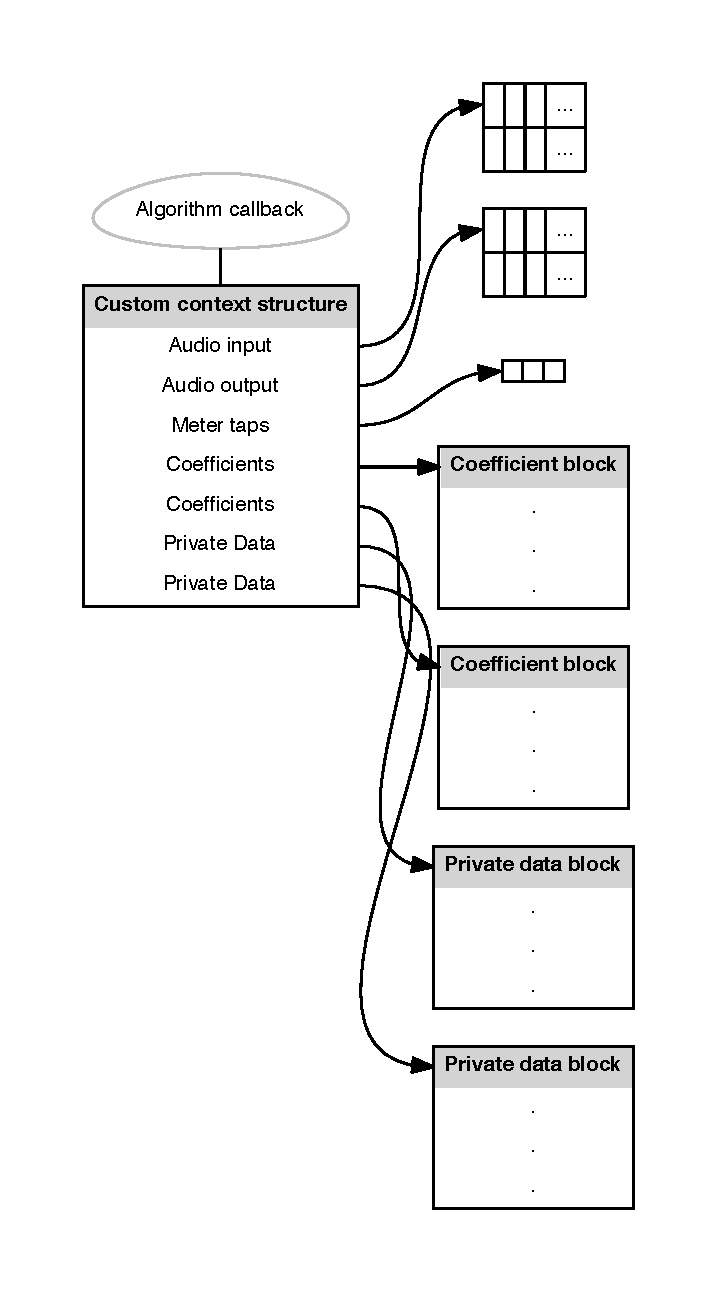
\includegraphics[width=\textwidth,height=\textheight/2,keepaspectratio=true]{dot_aax_alg_context}}
\end{DoxyImageNoCaption}


 When the A\+A\+X host calls a plug-\/in\textquotesingle{}s algorithm callback, it provides a block of memory describing the state of the plug-\/in. This block of memory, known as the algorithm\textquotesingle{}s {\itshape context}, can be thought of as the algorithm\textquotesingle{}s interface to the outside world\+: when another part of the plug-\/in interacts with the algorithm, it does so by posting information to the algorithm\textquotesingle{}s context.


\begin{DoxyCode}
\textcolor{comment}{//==============================================================================}
\textcolor{comment}{// Component context definitions}
\textcolor{comment}{//==============================================================================}

\textcolor{comment}{// Context structure}
\textcolor{keyword}{struct }SDemoDist\_Alg\_Context
\{
    int32\_t                 * mCtrlBypassP;                 \textcolor{comment}{// Coefficient message destination}
    \textcolor{keywordtype}{float}                   * mCtrlMixP;                    \textcolor{comment}{// Coefficient message destination}
    \textcolor{keywordtype}{float}                   * mCtrlInpGP;                   \textcolor{comment}{// Coefficient message destination}
    \textcolor{keywordtype}{float}                   * mCtrlOutGP;                   \textcolor{comment}{// Coefficient message destination}
    SDemoDist\_DistCoefs     * mCoefsDistP;                  \textcolor{comment}{// Coefficient message destination}
    SDemoDist\_FiltCoefs     * mCoefsFiltP;                  \textcolor{comment}{// Coefficient message destination}

    CSimpleBiquad           * mBiquads;                     \textcolor{comment}{// Private data}

    \textcolor{keywordtype}{float}*                  * mInputPP;                     \textcolor{comment}{// Audio signal input}
    \textcolor{keywordtype}{float}*                  * mOutputPP;                    \textcolor{comment}{// Audio signal output}
    \textcolor{keywordtype}{float}*                  * mMeterTapsPP;                 \textcolor{comment}{// Meter signal output}
\};
\end{DoxyCode}


 It is important to note that, in most circumstances, algorithm callbacks do not own their own memory. The algorithm and its memory is managed entirely by the host or shell environment, and relies on the host-\/provided context structure for all state information.

 If persistent memory is required, algorithms can register for block(s) of persistent state date via the \hyperlink{a00088_a125949841a13e97ff93fa321f2050433}{A\+A\+X\+\_\+\+I\+Component\+Descriptor\+::\+Add\+Private\+Data()} A\+P\+I (as in S\+Demo\+Dist\+\_\+\+Alg\+\_\+\+Context\+::m\+Biquads above.) A plug-\/in may store state data in the resulting {\itshape \char`\"{}private data\char`\"{}} context fields and this data will be restored by the host when the algorithm is next called. See the \hyperlink{a00327_alg_pd}{Persistent algorithm memory} section below for more information. 

 \hypertarget{a00327_alg_comm}{}\subsection{Communicating with the algorithm}\label{a00327_alg_comm}
 Plug-\/ins communicate with their algorithms via a buffered, host-\/managed message system. The host guarantees that messages posted to this system will be delivered to the applicable context field and that the algorithm\textquotesingle{}s context is up to date every time the component is entered.

 This system utilizes a static data routing scheme that is defined in the plug-\/in\textquotesingle{}s describe method. Once the routing scheme has been defined, the plug-\/in may post packets of data to its algorithm using \hyperlink{a00090_ae5dd2b5925dbc181513bca1c4ac5e716}{A\+A\+X\+\_\+\+I\+Controller\+::\+Post\+Packet()}.

 In order to reference the fields in its algorithm\textquotesingle{}s context, the plug-\/in\textquotesingle{}s host-\/side code uses unique identifiers generated with the \hyperlink{a00149_acf807247ecd6e5899dc9dc31644e9a1d}{A\+A\+X\+\_\+\+F\+I\+E\+L\+D\+\_\+\+I\+N\+D\+E\+X} macro\+:


\begin{DoxyCode}
\textcolor{keyword}{enum} EDemoDist\_Alg\_PortID
\{
     eAlgPortID\_BypassIn                    = \hyperlink{a00149_acf807247ecd6e5899dc9dc31644e9a1d}{AAX\_FIELD\_INDEX} (SDemoDist\_Alg\_Context, 
      mCtrlBypassP)
    ,eAlgPortID\_MixIn                       = \hyperlink{a00149_acf807247ecd6e5899dc9dc31644e9a1d}{AAX\_FIELD\_INDEX} (SDemoDist\_Alg\_Context, 
      mCtrlMixP)
    ,eAlgPortID\_InpGIn                      = \hyperlink{a00149_acf807247ecd6e5899dc9dc31644e9a1d}{AAX\_FIELD\_INDEX} (SDemoDist\_Alg\_Context, 
      mCtrlInpGP)
    ,eAlgPortID\_OutGIn                      = \hyperlink{a00149_acf807247ecd6e5899dc9dc31644e9a1d}{AAX\_FIELD\_INDEX} (SDemoDist\_Alg\_Context, 
      mCtrlOutGP)
    ,eAlgPortID\_CoefsDistIn                 = \hyperlink{a00149_acf807247ecd6e5899dc9dc31644e9a1d}{AAX\_FIELD\_INDEX} (SDemoDist\_Alg\_Context, 
      mCoefsDistP)
    ,eAlgPortID\_CoefsFilterIn               = \hyperlink{a00149_acf807247ecd6e5899dc9dc31644e9a1d}{AAX\_FIELD\_INDEX} (SDemoDist\_Alg\_Context, 
      mCoefsFiltP)

    ,eAlgFieldID\_Biquads                    = \hyperlink{a00149_acf807247ecd6e5899dc9dc31644e9a1d}{AAX\_FIELD\_INDEX} (SDemoDist\_Alg\_Context, 
      mBiquads)

    ,eDemoDist\_AlgFieldID\_AudioIn           = \hyperlink{a00149_acf807247ecd6e5899dc9dc31644e9a1d}{AAX\_FIELD\_INDEX} (SDemoDist\_Alg\_Context, 
      mInputPP)
    ,eDemoDist\_AlgFieldID\_AudioOut          = \hyperlink{a00149_acf807247ecd6e5899dc9dc31644e9a1d}{AAX\_FIELD\_INDEX} (SDemoDist\_Alg\_Context, 
      mOutputPP)
    ,eAlgFieldID\_MeterTaps                  = \hyperlink{a00149_acf807247ecd6e5899dc9dc31644e9a1d}{AAX\_FIELD\_INDEX} (SDemoDist\_Alg\_Context, 
      mMeterTapsPP)
\};
\end{DoxyCode}


 See \hyperlink{a00326}{Description callback} for more information about registering context fields and defining a plug-\/in\textquotesingle{}s message routing scheme. 

 \hypertarget{a00327_alg_initialization}{}\subsection{Algorithm initialization}\label{a00327_alg_initialization}
 The following events occur before the A\+A\+X host begins calling a plug-\/in\textquotesingle{}s algorithm\+:

 \begin{DoxyItemize}
\item The Effect\textquotesingle{}s \hyperlink{a00328}{data model} is initialized \item An initial call to \hyperlink{a00061_a6e87e40d42c7431e52ae5ebd4f631964}{A\+A\+X\+\_\+\+I\+Effect\+Parameters\+::\+Reset\+Field\+Data()} is made for each private data block in the algorithm. \item An initial call to \hyperlink{a00061_a083265b008921b6114ede387711694b7}{A\+A\+X\+\_\+\+I\+Effect\+Parameters\+::\+Generate\+Coefficients()} is made and coefficient packets are dispatched to each of the algorithm\textquotesingle{}s data ports based on the default model state. \item All packets are delivered and initial algorithm context state is set \item If one has been registered, the algorithm\textquotesingle{}s optional initialization callback is called with the default context \item (Algorithmic processing begins)\end{DoxyItemize}
\hypertarget{a00327_alg_initialization_private_data}{}\subsubsection{Private data initialization}\label{a00327_alg_initialization_private_data}
 To initialize an algorithm\textquotesingle{}s private data blocks, \hyperlink{a00061_a6e87e40d42c7431e52ae5ebd4f631964}{A\+A\+X\+\_\+\+I\+Effect\+Parameters\+::\+Reset\+Field\+Data()} is called on the host for each block in the algorithm. The host uses this method to acquire a default initialized memory block for each private data port, which is then copied into the algorithm\textquotesingle{}s memory pool and provided to its context.

 The default implementation of this method in \hyperlink{a00018_accef965824c9b158cafb65e59e216b6a}{A\+A\+X\+\_\+\+C\+Effect\+Parameters} will initialize the data to zero.

 \begin{DoxySeeAlso}{See also}
\hyperlink{a00327_alg_pd}{Persistent algorithm memory}
\end{DoxySeeAlso}
\hypertarget{a00327_alg_initialization_optional_callback}{}\subsubsection{Optional initialization callback}\label{a00327_alg_initialization_optional_callback}
 If any additional initialization or de-\/initialization steps are required for proper operation of the algorithm, an optional initialization routine may be registered and associated with the algorithm\textquotesingle{}s processing callback. This initialization routine will be called in the same device / memory space as the algorithm\textquotesingle{}s processing context. The initialization callback is provided with the algorithm\textquotesingle{}s default context and is called both before every new instance of the Effect begins its algorithm render callbacks and before every instance is destroyed.

 This initialization routine is provided in \hyperlink{a00326}{Describe} as an argument to the platform\textquotesingle{}s {\ttfamily Add\+Process\+Proc} registration method\+:

 \begin{DoxyItemize}
\item \hyperlink{a00088_a1c069508cf54a523905c8160ebf628ad}{A\+A\+X\+\_\+\+I\+Component\+Descriptor\+::\+Add\+Process\+Proc\+\_\+\+Native()} \item \hyperlink{a00088_aa8443e720e48046444a2e9f712f0864b}{A\+A\+X\+\_\+\+I\+Component\+Descriptor\+::\+Add\+Process\+Proc\+\_\+\+T\+I()}\end{DoxyItemize}
\begin{DoxyRefDesc}{Host Compatibility Notes}
\item[\hyperlink{a00380__compatibility_notes000002}{Host Compatibility Notes}]As of Pro Tools 10.\+2.\+1 an algorithm\textquotesingle{}s initialization calllback routine will have up to 5 seconds to execute.\end{DoxyRefDesc}


 \begin{DoxySeeAlso}{See also}
\hyperlink{a00163_a3963a850079d3186e08c97a1a4d0ef1c}{A\+A\+X\+\_\+\+C\+Instance\+Init\+Proc}
\end{DoxySeeAlso}


 \hypertarget{a00327_alg_processing}{}\subsection{Algorithm processing}\label{a00327_alg_processing}
 Once the algorithm has been initialized and processing begins, the algorithm function is called regularly by the host audio engine. The algorithm may read the context data provided by the host and is responsible for writing data to all of the samples in its output buffers each time it is executed.

 \begin{DoxyNote}{Note}
The data in an algorithm\textquotesingle{}s output buffers is not initialized before the algorithm is called, thus the algorithm must always write data into all output samples. This is to ensure equivalent behavior between all platforms, some of which do not have the resource budget to pre-\/initialize output data buffers.
\end{DoxyNote}


 \hypertarget{a00327_alg_pd}{}\subsection{Persistent algorithm memory}\label{a00327_alg_pd}
 An A\+A\+X plug-\/in algorithm may contain one or more {\itshape private data} ports in its context. These are the only context fields in which an algorithm may store persistant state data.

\hypertarget{a00327_alg_pd_characteristics}{}\subsubsection{Private memory characteristics}\label{a00327_alg_pd_characteristics}
 Each private data port is a pointer to a preallocated block of memory. The size of each port is defined during Describe when the port is registered. On D\+S\+P systems, the plug-\/in may request that the data block be placed in the chip\textquotesingle{}s external memory.

 Once private data is allocated by the plug-\/in host or D\+S\+P shell, it will not be relocated or re-\/allocated until the algorithm is destroyed (see \hyperlink{a00327_alg_initialization_optional_callback}{Optional initialization callback})

\hypertarget{a00327_alg_pd_registration}{}\subsubsection{Private data port registration}\label{a00327_alg_pd_registration}
 Private data ports are registered during Describe via \hyperlink{a00088_a125949841a13e97ff93fa321f2050433}{A\+A\+X\+\_\+\+I\+Component\+Descriptor\+::\+Add\+Private\+Data()}. This method defines the size of the data block that will be allocated as well as an initialization callback with format \hyperlink{a00163_adfb5d89b9d957c541fc98fe42bc050c4}{A\+A\+X\+\_\+\+C\+Init\+Private\+Data\+Proc}.

\hypertarget{a00327_alg_pd_init}{}\subsubsection{Private data initialization}\label{a00327_alg_pd_init}
 \hyperlink{a00061_a6e87e40d42c7431e52ae5ebd4f631964}{A\+A\+X\+\_\+\+I\+Effect\+Parameters\+::\+Reset\+Field\+Data()} is called on the host for both Native and D\+S\+P plug-\/ins. For D\+S\+P plug-\/ins, the initialized data block is copied to the D\+S\+P by the A\+A\+X host following the initialization callback. The initialization callbacks for a plug-\/in\textquotesingle{}s private data blocks are called after all host modules have been initialized and before the algorithm\textquotesingle{}s optional initialization callback.

 \begin{DoxySeeAlso}{See also}
\hyperlink{a00327_alg_initialization}{Algorithm initialization}
\end{DoxySeeAlso}
\hypertarget{a00327_alg_pd_comm}{}\subsubsection{Private data communication}\label{a00327_alg_pd_comm}
 It is possible to transfer data to and from the algorithm\textquotesingle{}s private data blocks using the \hyperlink{a00111}{A\+A\+X\+\_\+\+I\+Private\+Data\+Access} interface, which is available in a Timer\+Wakeup context through the \hyperlink{a00097}{A\+A\+X\+\_\+\+I\+Effect\+Direct\+Data} interface. For more information about this A\+P\+I, see auxinterface\+\_\+directdata\+\_\+privatedataaccess.



 \hypertarget{a00327_alg_examp}{}\subsection{Example algorithm callback}\label{a00327_alg_examp}
 As a final example, the code below describes a simple audio processing component. The component\textquotesingle{}s context contains one message pointer to receive incoming \char`\"{}gain\char`\"{} parameter values, as well as one audio data input, \char`\"{}pd\+I\char`\"{}, and one audio data output, \char`\"{}pd\+O\char`\"{}. Additionally there is a message pointer to receive \char`\"{}bypass\char`\"{} on/off values. The host calls the component each time a new input sample buffer must be processed, and each time the component is called the host ensures that all context fields are up-\/to-\/date.


\begin{DoxyCode}
\textcolor{keywordtype}{void} \hyperlink{a00149_aaa22112139aa627574b1ef562f579d43}{AAX\_CALLBACK} MyPlugIn\_AlgorithmProcessFunction(
    SMyPlugIn\_Alg\_Context * \textcolor{keyword}{const}   inInstancesBegin [],
    \textcolor{keyword}{const} \textcolor{keywordtype}{void} *                    inInstancesEnd)
    \{

        \textcolor{comment}{// Get a pointer to the beginning of the memory block table}
        SMyPlugIn\_Alg\_Context* AAX\_RESTRICT instance = inInstancesBegin [0];

        \textcolor{comment}{//--------- Iterate over plug-in instances ---------//}
        \textcolor{keywordflow}{for} (SMyPlugIn\_Alg\_Context * \textcolor{keyword}{const} * walk = inInstancesBegin; walk < inInstancesEnd; ++walk)
        \{
            instance = *walk;

            \textcolor{comment}{//--------- Retrieve instance-specific information ---------//}
            \textcolor{comment}{//}
            \textcolor{keyword}{const} SMyPlugIn\_CoefsGain* \textcolor{keyword}{const} AAX\_RESTRICT   coefsGainP =    instance->mCoefsGainP;  \textcolor{comment}{//
       Input (const)}
            \textcolor{keyword}{const} int32\_t   bypass      = *instance->mCtrlBypassP; 
            \textcolor{keyword}{const} \textcolor{keywordtype}{float}     gain        = coefsGainP->mGain;

            \textcolor{comment}{//--------- Run processing loop over each input channel ---------//}
            \textcolor{comment}{//}
            \textcolor{keywordflow}{for} (\textcolor{keywordtype}{int} ch = 0; ch < kNumChannelsIn; ch++) \textcolor{comment}{// Iterate over all input channels}
            \{

                \textcolor{comment}{//--------- Run processing loop over each sample ---------//}
                \textcolor{comment}{//}
                \textcolor{keywordflow}{for} (\textcolor{keywordtype}{int} t = 0; t < kAudioWindowSize; t++)
                \{
                    \textcolor{keywordtype}{float}* \textcolor{keyword}{const} AAX\_RESTRICT pdI = instance->mInputPP [ch];
                    \textcolor{keywordtype}{float}* \textcolor{keyword}{const} AAX\_RESTRICT pdO = instance->mOutputPP [ch];

                    \textcolor{keywordflow}{if} ( pdI && pdO )
                    \{
                        pdO [t] = gain * pdI [t];
                        \textcolor{keywordflow}{if} (bypass) \{ pdO [t] = pdI [t]; \} 
                    \}
                \} \textcolor{comment}{// Go to the next sample}
            \} \textcolor{comment}{// Go to next channel}
        \} \textcolor{comment}{// End instance-iteration loop}
    \}
\end{DoxyCode}




 \hypertarget{a00327_alg_porttypes}{}\subsection{Port Types and Behavior}\label{a00327_alg_porttypes}
In this section, we will examine the various kinds of ports that can be used by the algorithm component in an A\+A\+X plug-\/in\+: 
\begin{DoxyEnumerate}
\item Standard message input  
\item Internal state storage  
\item Metering output  
\item Environment variable retrieval  
\item Other functionality enhancement  
\end{DoxyEnumerate}

\hypertarget{a00327_subsection__standard_message_input}{}\subsubsection{Standard message input}\label{a00327_subsection__standard_message_input}
Most ports will function as pointers to incoming data. This data can have any type. For example, an algorithm\textquotesingle{}s context may include a port of type float$\ast$ to receive incoming float data and another port of type {\ttfamily S\+My\+Custom\+Structure}$\ast$ to receive incoming {\ttfamily S\+My\+Custom\+Structure} data.

Like all registered context fields, input ports are managed by the hosting environment such that they always point to the most recently received data at the time that the algorithm callback is entered. The algorithm may not store or alter data in a standard message input port\+: this data is available as read-\/only input. If data is stored in the space allocated for the port\textquotesingle{}s data then the result will be undefined behavior.

To define a standard message input port, a plug-\/in should call \hyperlink{a00088_a230293b9f6bb413626cd487ca501df75}{A\+A\+X\+\_\+\+I\+Component\+Descriptor\+::\+Add\+Data\+In\+Port()}.

\hypertarget{a00327_subsection__internal_state_storage}{}\subsubsection{Internal state storage}\label{a00327_subsection__internal_state_storage}
Most plug-\/ins require local data to be accessible to their algorithms. These may be static data, such as lookup tables, or dynamic data, such as coefficient smoothing history or delay lines. In the Demo\+Dist sample plug-\/in, {\ttfamily S\+Demo\+Dist\+\_\+\+Alg\+\_\+\+Context\+::m\+Biquads} is an example of this type of port\+: it is not modified by any other component and {\ttfamily Demo\+Dist\+\_\+\+Algorithm\+Process\+Function()} relies on the {\ttfamily m\+Biquads} data persisting between processing calls.

A component that has registered a private data field is given access to a block of private data. Although the memory in this block will be allocated by the host, its data is fully owned by the component. Because this data is considered private to its parent component, other components cannot overwrite or target this data. Plug-\/ins that need to transmit data directly between their algorithms\textquotesingle{} private data ports and their other modules may use the \hyperlink{a00097}{A\+A\+X\+\_\+\+I\+Effect\+Direct\+Data} interface, which provides an A\+P\+I for reading from or writing to this data from outside of the algorithm callback.

The plug-\/in\textquotesingle{}s data model includes an initialization function that is called by the A\+A\+X host at the time of plug-\/in instantiation and \char`\"{}reset\char`\"{} events. This initialization method is called on the host for both Native and D\+S\+P plug-\/ins. Since this method is part of the plug-\/in\textquotesingle{}s data model, it has direct access to plug-\/in state information.

\hypertarget{a00327_subsection__metering_output}{}\subsubsection{Metering output}\label{a00327_subsection__metering_output}
Plug-\/in metering ports are populated with an array of float values, or \textquotesingle{}taps\textquotesingle{}. One tap is provided per plug-\/in meter. The algorithm writes per-\/buffer peak values to this port and the A\+A\+X host applies standardized ballistics to these values. Both raw and processed meter values are available to the plug-\/in\textquotesingle{}s G\+U\+I.

\hypertarget{a00327_subsection__environment_variable_retrieval}{}\subsubsection{Environment variable retrieval}\label{a00327_subsection__environment_variable_retrieval}
Another use of ports is to receive data from the A\+A\+X host describing the execution environment. For example, an algorithm may include a port to receive the number of samples in its processing window or the sample rate. These services are provided automatically by the host once the component registers ports for them.

\hypertarget{a00327_subsection__other_functionality_enhancement}{}\subsubsection{Other functionality enhancement}\label{a00327_subsection__other_functionality_enhancement}
An algorithm component may use ports to gain additional functionality that is provided by the host. For example, an algorithm that will be compiled for accelerated environments may take advantage of the T\+I chip\textquotesingle{}s Direct Memory Access functionality by registering a D\+M\+A port. The host will then allow this port to access memory directly using \hyperlink{a00288}{A\+A\+X}\textquotesingle{}s D\+M\+A A\+P\+Is.



 \hypertarget{a00327_alg_seealso}{}\subsection{Additional Information}\label{a00327_alg_seealso}
 For information about optional features for the algorithm processing callback, see the following \hyperlink{a00332}{Additional A\+A\+X features} documentation\+:

 \begin{DoxyItemize}
\item \hyperlink{a00340}{Direct Memory Access} \item \hyperlink{a00341}{Background processing callback}\end{DoxyItemize}
 Collaboration diagram for Real-\/time algorithm callback\+:
\nopagebreak
\begin{figure}[H]
\begin{center}
\leavevmode
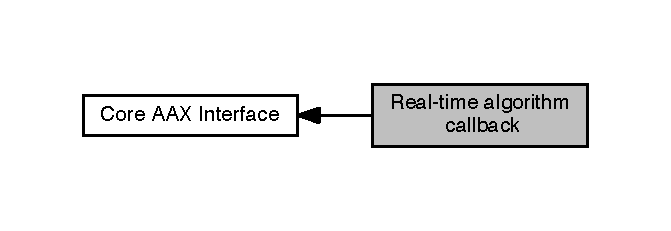
\includegraphics[width=322pt]{a00327}
\end{center}
\end{figure}
